\documentclass[hyperref,UTF8]{ctexart}
\usepackage{CJK}
\usepackage{indentfirst}
\usepackage{amsfonts}
\usepackage{amsmath}
\usepackage{amssymb}
\usepackage{amsthm}
\usepackage{graphicx}
\usepackage{geometry}
\usepackage{titlesec}
\usepackage[colorlinks, citecolor=black,hyperfootnotes=true]{hyperref}
\usepackage{fancyhdr}
\usepackage{setspace}
\begin{document}
\title{Sudoku}
\author{Zhang Xilin 2016050022}
\date{Sep 2, 2017}
\maketitle

\vspace {2cm}


\newpage

\tableofcontents

\newpage

\section{功能实现}
    该程序在主界面中设有,开始游戏,选择关卡,退出。
    分别对应游戏的第一关,选择关卡界面以及退出程序。
    在游戏界面中设有各类功能按钮,且所有承载重要数据的界面可随意更改大小(每个界面有各自的最小尺寸)
    其各类界面效果如下图:

\begin{center}
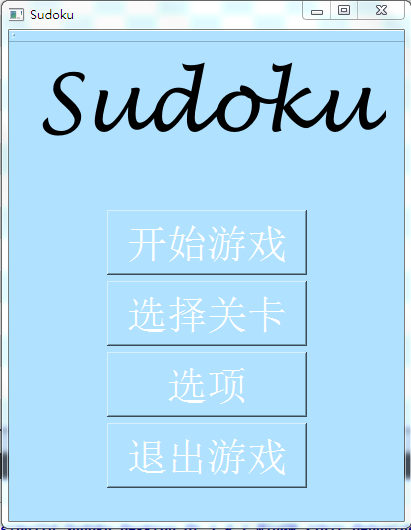
\includegraphics[width=4in]{theme.PNG}
\end{center}

\begin{center}
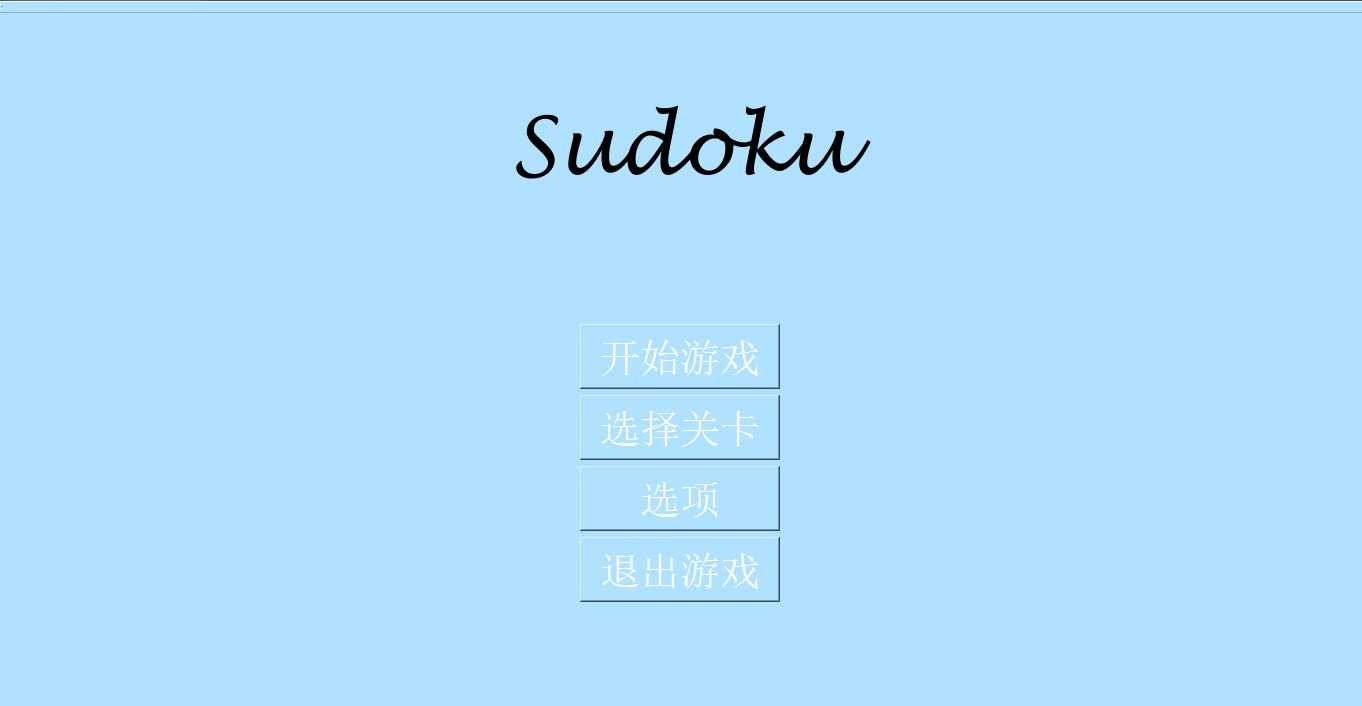
\includegraphics[width=4in]{theme1.PNG}
\end{center}

\begin{center}
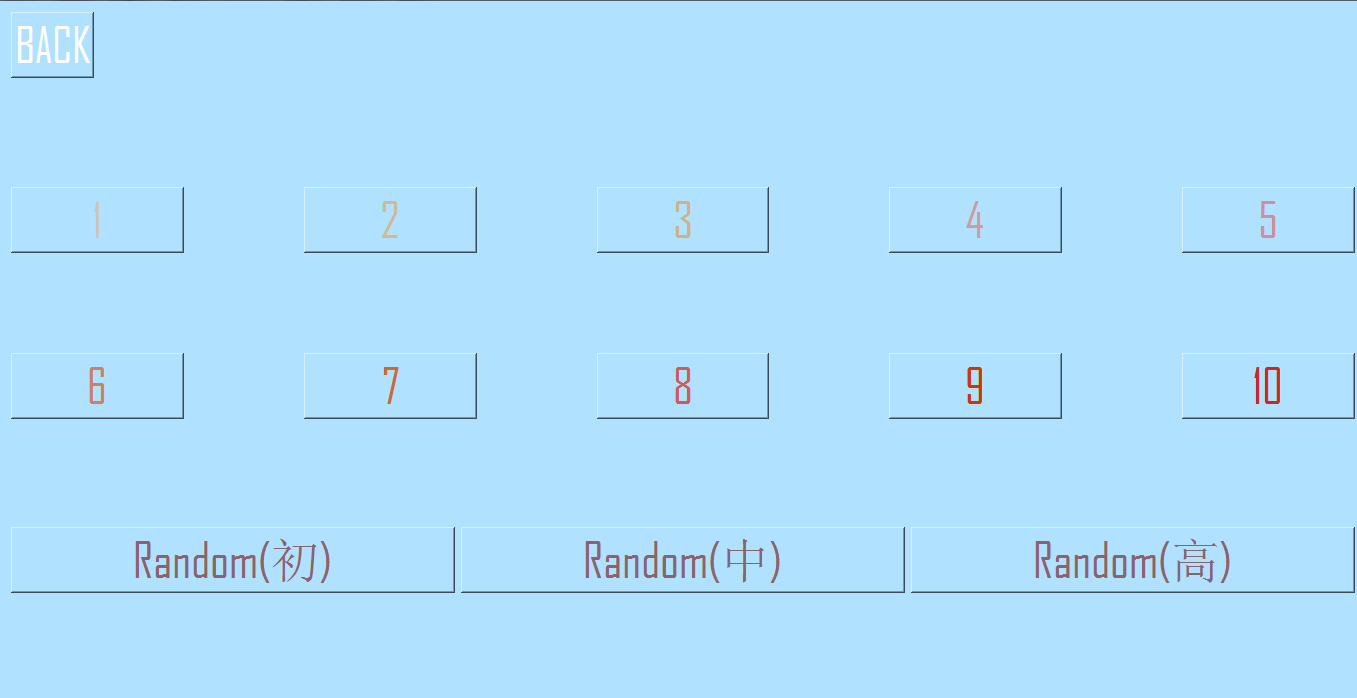
\includegraphics[width=4in]{sel.PNG}
\end{center}

\begin{center}
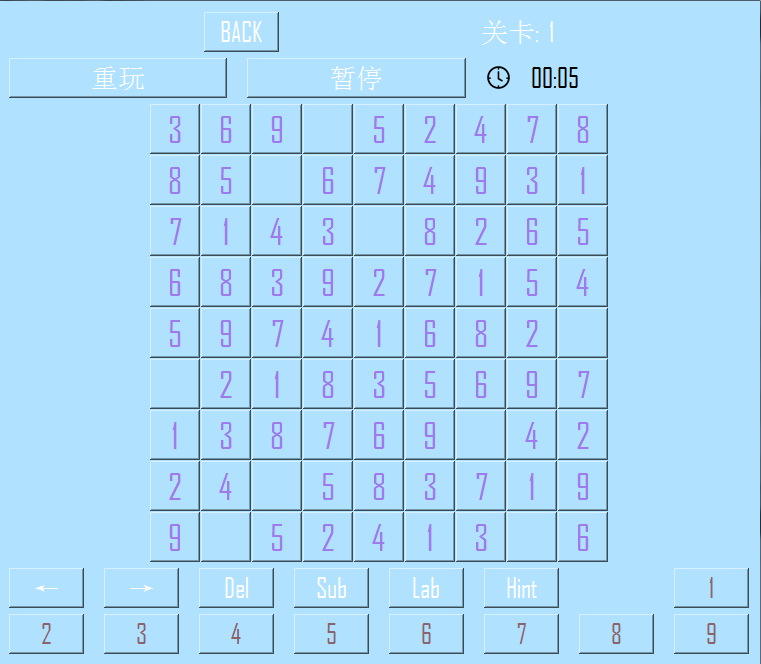
\includegraphics[width=4in]{game.PNG}
\end{center}

\begin{center}
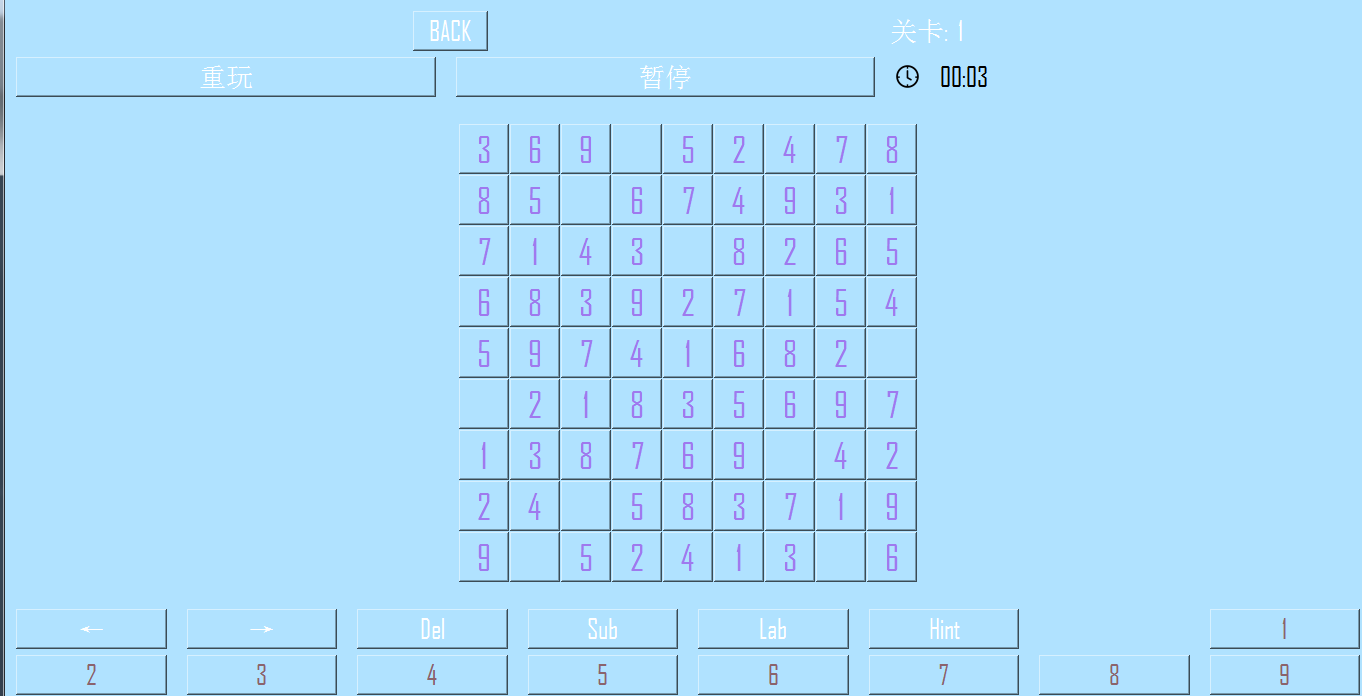
\includegraphics[width=4in]{game1.PNG}
\end{center}

\begin{center}
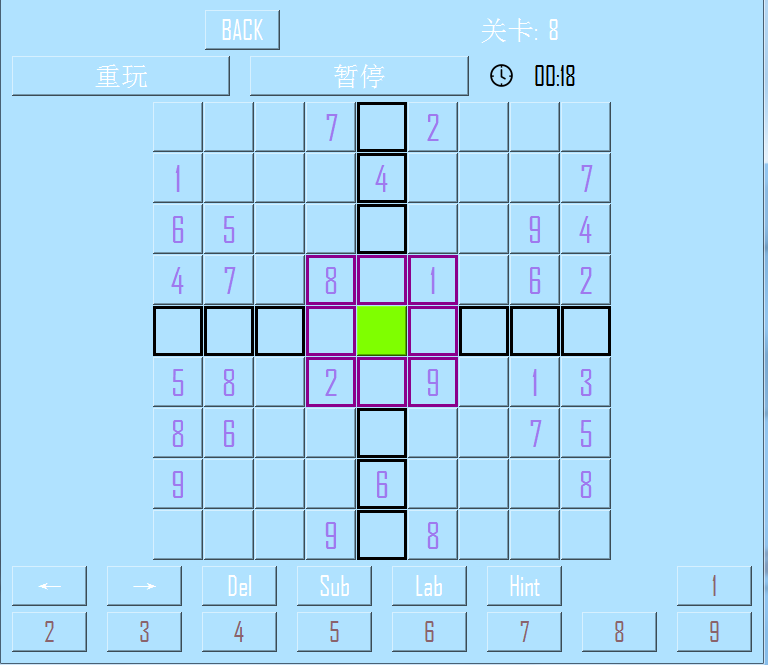
\includegraphics[width=4in]{click.PNG}
\end{center}

\begin{center}
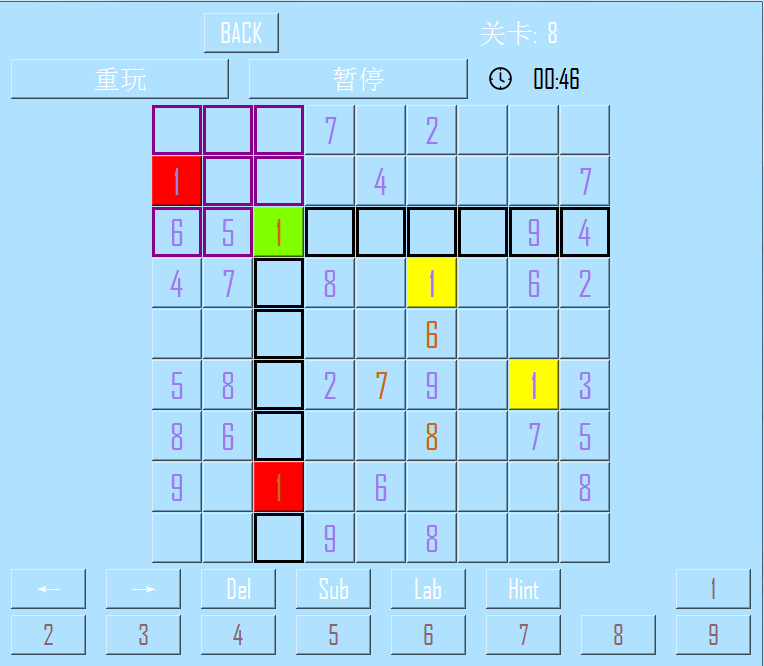
\includegraphics[width=4in]{same.PNG}
\end{center}

\begin{center}
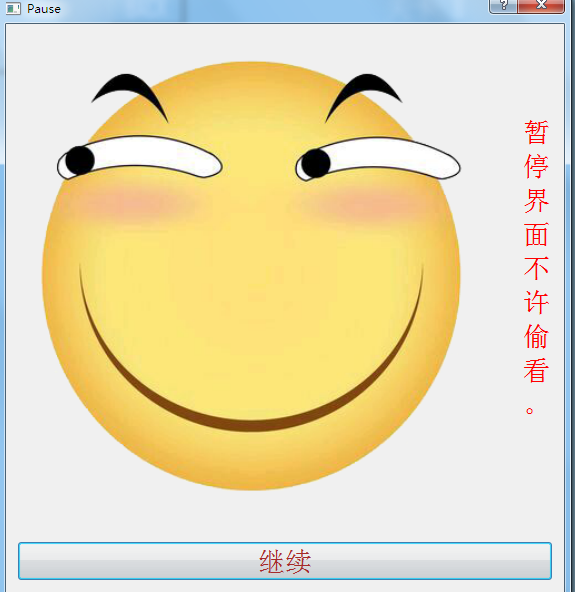
\includegraphics[width=4in]{pause.PNG}
\end{center}

    详细功能细节可运行程序查看。

    该程序的框架分为一个显示主界面的类MainWindow,该类中存放了其他界面的实例化对象
    并在需要的时候进行克重窗口的切换。

    在选择关卡的前10个关卡为默认写死在代码里的关卡,下面的三个等级的Random按钮,则是
    随机生成的挖出10个,20个,30个空的样例。
    对每个随机的样例都是基于一个种子样例实现的。
    种子样例代表一个符合数组规则且没有空的数组。
    之后对这个样例施加特殊的行列变换还是依然满足数独的规则的。
    之后对变换得到的样例随机挖空最终得到结果。


    该游戏通过先点击一个可以修改的格子,然后点击下面的数字即可进行输入,每个格子可以
    容纳最多9个数字,如果在一个格子中点击已经存在的数字,则不会进行添加。
    每次点击格子的同时会自动将其所属的九宫格,以及所在的行列加上边框样式,
    并对不满足规则的格子加以红色背景显示,相同内容的格子也会以黄色背景示意。

    左右箭头的按钮可以达到撤销以及恢复的效果。

    Del按钮可以删除指定格子的所有备选数字。

    Sub按钮将所填答案提交,正确的话就会显示一个对话框提示。同时暂停计时器。

    Hint按钮可以显示答案。
    该按钮调用的数独求解方法是通过暴力DFS得到的。

    重玩可以将本局游戏置为刚开始的状态。

    暂停按钮显示一个对话框并暂停计时器,点击出现的对话框中的继续按钮可以开始计时器。

\newpage

\section{Class}
\subsection{MainWindow}
    主要成员变量:

    game:                             Game 类的实例化对象,存放游戏界面。

    select:                           Select类的实例化对象,存放选择关卡的界面。

    主要函数的功能为页面切换。



\subsection{Game}
    Game类为最重要且最核心的一个类,其中存放了大量游戏所需数据。

    主要成员变量:

    numButton:                        记录每个格子中数字的数量。

    numEnabled:                       记录每个格子书否是只读属性的。

    levelSet:                         关卡的参数。

    Level:                            写死在代码中前10关的数据。

    Un/RedoList:                      存放撤销恢复的数据。

    record:                           最近一次鼠标与九宫格内按钮互动的位置。

    gen:                              Generator的实例化对象,用于生成Random关卡的数据。

    pause:                            Pause的实例化对象,存放Pause界面。

    主要成员函数:

    check():                          点击Sub按钮调用的函数,检查结果是否满足规则。

    init():                           重玩按钮调用的函数,初始化界面。

    SameGrid(int, int):               对所选按钮具有相同内容的设置样式。

    void onpushButtonclicked():        关闭此页面。

    void ongridbuttonclicked(int):    选中九宫格的按钮,触发样式设计,并将
    点击位置存入record。

    void showtime():                  显示时间。

    void onreplayclicked():           重新开始。

    void onnumclicked(int):           对所选按钮填入数字。
    每次点击将之前数独所有的状态信息存入UndoList用于撤销。

    void onstopTimerclicked():        停止计时器所调用的函数。

    void onSubmitclicked():           调用check函数判断是否正确。

    void onUndoclicked():             点击实现撤销至上一状态,并将点击撤销之前的状态存入
    RedoList,并对UndoList popback。

    void onRedoclicked():             点击实现恢复效果,并将点击之前的状态存入UndoList,
    并对RedoList popback。

    void Hintclick():                 点击Hint按钮调用此函数。
    该函数调用Solver实例化对象的solve方法进行对当前数独的求解,
    并自动填充到正确位置。

    void onDelclicked();               将所选button的text属性设为空,同时将numButton设为0.





\subsection{Generator}
    创建随机的数独样例。

    主要成员变量:

    ranSeed: 初始的种子样例。

    Difficulty: 空格的数量。

    tmp: 承载样例的中间变量。

    主要成员函数:

    void chooseSeed(): 选择第几个种子作为实验样例。

    void changeRow(): 行变换。

    void changeCol(): 列变换。

    void changeGri(): 区块变换。

    void ranDig(): 随机挖洞。

    void check():检查满足数组规则.

    void reCot(): 随机进行行列变化,重构。

    Data getAns():得到数独结果数据。

    void setDif(int): 设置难度。





\subsection{Pause}
    Pause界面数据。



\subsection{Select}

    关卡选择的界面,进行各种页面切换。

\newpage

\subsection{Solver}

    利用DFS的方法求解数独。


\subsection{State}

    该类用于存放数独的各种状态。

    style:所有格子的样式。

    text: 所有格子的内容。
·
    numButton:所有格子中数字的数量。

    numEnabled: 所有格子是否是只读属性的。

    record:点击按钮的坐标。


\subsection{win}
    赢了之后所显示的页面。

\newpage

\subsection{心路历程}

    在开始的时候,发现设置的按钮会被钉死在像素位置,不会随着窗口大小的变化而自动适应屏幕。
    在利用Designer设计框架并加上弹簧之后实现了这一目的。

    在每次点击九宫格的某一个格子时,都需要重新设置其他格子的样式。同时,在调用setstylesheet设置样式时会覆盖之前的样式。
    即时将原来的样式保存并直接使用也同样会涉及到很多样式重置的问题,这就很不舒服。

    同时再设计配色的时候也感到比较无力,想象的总比做出来的要好很多。

    最后实现了所有的基本功能之后才松了一口气。




\end{document}
